\chapter{Analyse et spécification des besoins}
\label{sec:unchapitre}

\begin{fquote}Dans ce chapitre, j’aborde les phases d’analyse et de spécification des besoins du projet, dans le but d’avoir une vision globale claire du comportement du projet ainsi que les attentes des utilisateurs.
 \end{fquote}
\begin{figure}[ht]
	\centering
	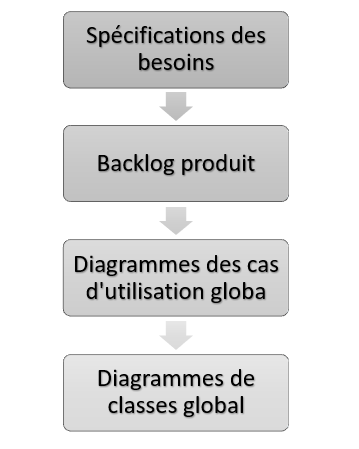
\includegraphics[width=8cm,height=9cm]{Sanstllitre2.png}
	\caption{Section de chapitre 2.}
	\label{fig:Section de chapitre 2}
\end{figure}
\FloatBarrier
\clearpage

\section{Spécifications des besoins}

La spécification des besoins va nous permettre d’avoir une meilleure approche des utilisateurs, des fonctionnalités et de la relation entre les deux. Elle sera sous forme de besoins. Pour cela nous allons procéder comme ceci :
\begin{itemize}
	\item Identification des acteurs du nouveau système.
	\item Identification des besoins fonctionnels.
	\item Identification des besoins non fonctionnels .
\end{itemize}

\subsection{Le processus d’apprentissage}

\begin{itemize}
	\item \underline{Apprentissage }: L’apprentissage est décrit comme un ensemble de mécanismes menant à
	l’acquisition de savoir, savoir -faire, savoir-être ou de connaissances.
	Dans ce processus l’acteur de l’apprentissage est appelé apprenant son rôle et d’acquérir la
	connaissance qui peut être opposé à l’enseignement dont le but est de dispenser des connaissances
	et savoirs. 
	
	
	\item  \underline{ Enseignement} : L’enseignement est l’action de transmettre des connaissances nouvelles ou
	savoirs à un apprenant (instruire et endoctriner tout en respectant certaines règles). Il s’agit du
	système et de la méthode d’enseigner, composée par tout un ensemble de connaissances, de
	principes et d’idées transmis à quelqu’un.
	L’enseignement constitue un composant de l’éducation, ce dernier terme beaucoup plus
	général, correspond à la formation globale d’un individu, à divers niveaux (au niveau religieux, moral,
	social, technique, scientifique, médical, etc.) 	
	\item \underline{ Didactique }: La didactique vient du grec qui signifie "enseigner", c’est la science qui a pour
	objet l’étude des méthodes et des pratiques de l’enseignement en général, ou de l’enseignement
	d’une discipline ou d’une matière particulière .
	Une méthode didactique c’est une méthode d’enseignement qui suit une approche
	scientifique ou style éducatif cohérente pour engager l’esprit de l’étudiant. Et on distingue :
	\begin{itemize}	
	\item[$\star$] La didactique générale qui s’intéresse à la conduite de la classe (cours magistraux,
	leçons dialoguées, travaux pratiques individuels ou collectifs, utilisation de manuels,
	etc.);
	\item[$\star$] La didactique spéciale qui s’intéresse à l’enseignement d’une discipline particulière
	pour une classe, un cycle d’études ou un ordre d’enseignement.
\end{itemize}
	\item \underline{ Le triangle didactique }: proposé par Jean Houssaye en 1988 comme modèle de
	compréhension du pédagogique. Il se compose des composantes principales d’un acte pédagogique
	(étudiant, savoir, enseignant) et les processus (apprendre, enseigner, former). De cela, il permet de faire des comparaisons entre les diverses situations pédagogiques  :
	\begin{figure}[ht]
		\centering
		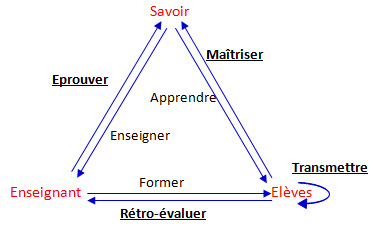
\includegraphics[width=14cm,height=8.5cm]{LetriangledejeanHoussaye.jpg}
		\caption{ Le triangle de jean Houssaye.}
		\label{fig: Le triangle de jean Houssaye}
	\end{figure}
	\FloatBarrier
	
	
		\begin{itemize}	
		\item[$\star$] Le processus Enseigner : axé de façon privilégiée sur la relation Savoir-Enseignant, et sur
		la transmission de ce savoir structurée par l’enseignant.
		\item[$\star$] Le processus Former : axé sur la liaison Enseignant-Former. Il correspond aux pédagogies
		centrées sur la formation humaine et sur la socialisation.
     	\item[$\star$]Le processus Apprendre : Il porte sur le rapport direct Savoir-Apprenant. Là, l’enseignant
    	devient l’organisateur de situations et de conditions externes d’apprentissage par
    	lesquelles il met en relation savoir et apprenant en jouant un rôle de médiateur.
	
     \end{itemize}
\end{itemize}







\clearpage

\subsection{Identification des acteurs}
Un acteur est une personne, un matériel ou un logiciel qui interagit avec le système. L’analyse du présent projet commence par une identification des acteurs agissants sur les différentes parties du système. Les acteurs présentés dans la figure \ref{fig:profiles} sont des employés du clients en plus du serveur  qui est la solution adoptée par le client pour la communication et le partage des informations entre ces systèmes et départements .

\begin{figure}[ht]
  \centering
  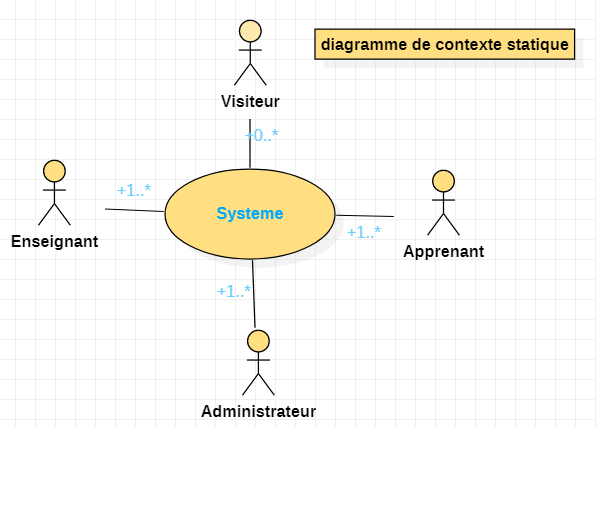
\includegraphics[width=14cm,height=8.5cm]{profiles}
  \caption{Héirarchie des profiles humaines.}
  \label{fig:profiles}
\end{figure}
\FloatBarrier
Le tableau \ref{actors} récapitule les acteurs en interaction avec le système en spécifiant le rôle de chacun avant de définir plus précisément leurs interactions avec le système en utilisant des diagrammes de cas d'utilisation.\\

\begin{table}[H]
\centering
\def\arraystretch{1.45}
\begin{tabular}{|c|c|}
\hline
\rowcolor{Gray} 
Acteur           & Fonction                                                                                                                                                                                                                                             \\ \hline
\rowcolor{LightCyan} 
Administrateur    & \begin{tabular}[c]{@{}c@{}} L’administrateur est la personne responsable de gérer la totalité du système.\\  \end{tabular} \\ \hline
\rowcolor{LightCyan} 



Enseignant & \begin{tabular}[c]{@{}c@{}} C’est un acteur principale qui interagit avec notre application.\\
C’est l’acteur qui a pour rôle de gérer les cours,\\ les travaux dirigés (TD) et les examens des
étudiants.\end{tabular}                   \\ \hline
\rowcolor{LightCyan} 



 
Apprenant & \begin{tabular}[c]{@{}c@{}}L’apprenant inscrit, il va pouvoir consulter \\les cours et faire les tests qui lui sont
	proposés.\\ L'apprenant peut avoir la possibilité de participer aux forums,\\ d'envoyer un
	message à un tuteur, \\à un autre apprenant ou même à l'administrateur.\\ Ainsi la possibilité
	de discussion en ligne avec le tuteur,\\ la modification de son profil et la consultation de
	sesrésultats.\end{tabular}                   \\ \hline
\rowcolor{LightCyan} 



Visiteur & \begin{tabular}[c]{@{}c@{}}N’importe quel visiteur qui \\veut télécharger des cours via un compte personnelle a
	condition \\ de faire les inscriptions pour avoir un compte.\end{tabular}                   \\ \hline
\rowcolor{LightCyan} 
\end{tabular}
\caption{Acteurs en interaction avec le système}
\label{actors}
\end{table}

\subsection{Les besoins fonctionnels}
Les besoins fonctionnels expriment une action que doit effectuer le système en réponse à une demande .\\
Les besoins principaux à couvrir par le système sont les suivants :\\
{\color{cyan} Si l’acteur est un Administrateur, il peut :
}

\begin{itemize}
	\item \underline{S’authentifier}  :l’Administarateur entre son « username » et son « password » avant d’accéder à l’application pour assurer la confidentialité des informations.
	\item \underline{Gérer les comptes des utilisateurs} : l’Administrateur peut ajouter des comptes pour les
	nouveaux Utilisateurs(Enseignant ou Etudiant) , modifier leurs informations et supprimer
	les comptes des anciens utilisateurs.
\end{itemize}
\clearpage
{\color{cyan}Si l’acteur est un Enseignant, il peut :}
\begin{itemize}
	\item \underline{Gérer les Matières} :l’Enseignant peut ajouter, modifier et supprimer les matières.
	\item  \underline{Gérer les Cours }:l’Enseignant peut ajouter, modifier et supprimer les cours.

	\item \underline{Gérer les Traveaux dirigés(TD) }:l’Enseignant peut ajouter,modifier et supprimer les Traveaux dirigés(TD).
	\item \underline{Gérer les Examens }:l’Enseignant peut ajouter des examens en choisissant une durée de
	temps determiné.
\end{itemize}
{\color{cyan}Si l’acteur est un Etudiant, il peut :}
\begin{itemize}
	\item \underline{Consulter les Cours} :l’Etudiant peut consulter et télecharger les cours.
	\item \underline{Consulter les Traveaux dirigés(TD) }:l’Etudiant peut consulter et télecharger les Traveaux
	dirigés(TD).
	\item \underline{Passer les Examens }:l’Etudiant peut passer les examens en respectant une durée de temps
	determinée.
\end{itemize}

\subsection{Les besoins non fonctionnels}
Les besoins non fonctionnels impressionne directement sur déroulement réelle de l’application. Ce sont des besoins techniques décrivant la majorité des contraintes (qu’on a déjà
approuvée dans le chapitre précèdent) auxquelles est soumis le système pour sa réalisation et
son bon fonctionnement. Pour cela l’ensemble des extensions à réaliser doivent respecter les besoins suivants :
%Les besoins non fonctionnels représentent les exigences implicites auquel le système doit répondre. Parmi ces besoins on cite :

\begin{itemize}
	\item \underline{La Sécurité} : La solution proposée permet à l’utilisateur une navigation sécurisée.
	Elle n’est accessible qu’avec une authentification.
	\item \underline{Ergonomie de l’interface }: L’ergonomie est un élément important de l’application : les
	écrans de saisie doivent être clairs, organisés avec cohérence, de façon à ce qu’une prise
	en main soit la plus rapide possible.
	\item \underline{
Maintenance }: L’une des plus importantes besoins de notre application est la facilité de
	modification pour s’adopter aux nouveaux besoins.
	\item \underline{Portabilité} : L’application doit être accessible via n’importe quel navigateur.

\end{itemize}

%\section{Analyse des besoins fonctionnels}
%L’analyse des besoins est une étape très importante dans le processus de l’étude et le développement des systèmes d’informations. Cette partie identifie l’ensemble des acteurs qui interagissent avec le système et définit l’ensemble des cas d’utilisation de ce dernier en se basant sur les diagrammes UML.
\section{Backlog produit}
Le Backlog produit est une liste ordonnée de tout ce qui pourrait être nécessaire dans un produit et constitue l’unique source d'exigences pour toutes les modifications apportées au produit. Le Product Owner est responsable du Backlog produit, y compris son contenu, sa disponibilité et son ordonnancement.\\
 Ses toutes premières moutures ne font qu’esquisser les besoins tels qu’initialement connus et compris. Le Backlog Produit évolue au fur et à mesure que le produit et le contexte dans lequel il sera utilisé évoluent. Le Backlog Produit est dynamique; il change constamment pour identifier ce que le produit requiert pour être approprié, compétitif et utile. Tant et aussi longtemps qu’un produit existe, son Backlog Produit correspondant existe.\\
 Les caractéristiques fonctionnelles sont appelées
 des histoires utilisateurs (user story). Les user stories sont caractérisés par :\\
\begin{itemize}[label=$\square$,leftmargin=* ,parsep=0cm,itemsep=0cm,topsep=0cm]
    \item \textit{\textbf{Identifiant}} Il détermine un identifiant unique pour l’histoire en question.\\
 	
 	\item \textit{\textbf{Description}}Elle décrit le besoin d’un acteur.\\
 	
 	\item \textit{\textbf{Critères d’acceptation}}À chaque user story sont associés des critères permettant au client
 	de tester l’histoire. Ces critères d’acceptation peuvent être formalisés, pour aller un peu plus
 	loin dans l’aide fournie à l’équipe que l’énoncé de ces critères.\\
 
 	\item \textit{\textbf{Estimation}}Est une estimation de la complexité, elle est une valeur entière qui appartient à la suite de Fibonacci.
 	 
 	
 	\item \textit{\textbf{Priorité}}  Les priorités sont utilisées pour définir l’ordre de réalisation, elles permettent de
 	constituer le flux de stories qui va alimenter l’équipe. Pour prioriser nos user stories, nous
 	avons pris en compte les critères suivant :
 	\begin{enumerate}
 		\item \textit{La valeur apportée (Business Value)}
 		\item \textit{La fréquence d’utilisation}
 		\item \textit{La réduction des risques}
 		\item \textit{L’incertitude sur des besoins des utilisateurs qu’un user story permettra de diminuer}
 		\item \textit{La contribution à la qualité. Les travaux visant à garantir la qualité du produit devraient être prioritaires}
 		\item \textit{Les dépendances entre stories}
 	\end{enumerate}
 	
Lors de la création de notre Backlog, nous avons essayé de produire des user stories qui respectent
les critères réunies dans le mot INVEST, c’est à dire
	\begin{itemize}	
\item[$\star$] Independant : Ne dépend de rien (réduire les liens entre items)
\item[$\star$] Negociable : Je n’ai pas une solution technique figée
\item[$\star$] Valuable : pour le client (a une valeur Business)
\item[$\star$] Estimable : Estimation en complexité
\item[$\star$] Small / Sized Appropriately : De petite taille (A définir en interne de l’entreprise)
\item[$\star$] Testable : Pour la validation de l’item
\end{itemize}
\end{itemize}
 \bigskip
 





\section{Diagrammes des cas d'utilisation global}
Le modèle des cas d’utilisation décrit les fonctionnalités d’un système d’un point de vue utilisateur, sous la forme d’actions et de réactions ; l’ensemble des fonctionnalités est déterminé en examinant les besoins fonctionnels de tous les utilisateurs potentiels.\\
Ainsi, pour construire notre modèle, nous allons organiser les cas d’utilisation et les regrouper en ensembles fonctionnels cohérents. Pour ce faire, nous utilisons le concept général d’UML, le package.


Ce diagramme illustre le cas d’utilisation générale de notre système. Ces cas d’utilisation seront par la suite expliqués en détaille. (voir la figure \ref{fig:UseCaseAdmin}):
\begin{figure}[ht]
  \centering
  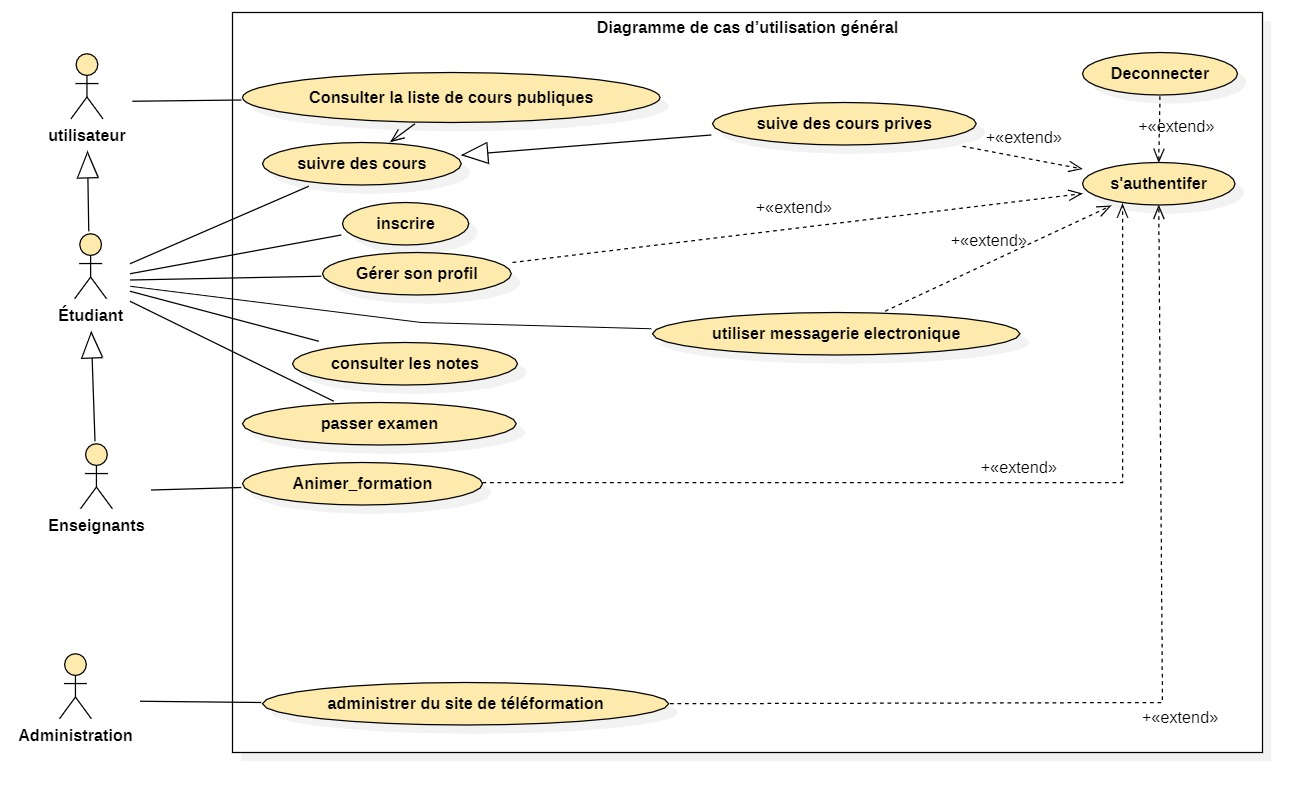
\includegraphics[width=18cm,height=9cm]{Diagrammedecasdutilisationgénéra.jpg}
  \caption{Les cas d'utilisation global.}
  \label{fig:UseCaseAdmin}
\end{figure}
\FloatBarrier

     
\section{Diagrammes de classes global}
Le diagramme de classes est un schéma utilisé en génie logiciel pour présenter les classes et les interfaces des systèmes ainsi que les différentes relations entre celles ci. Ce diagramme fait
partie de la partie statique d’UML car il fait abstraction des aspects temporels et dynamiques.
Une classe est un ensemble de fonctions et de données (attributs) qui sont liées ensembles par un champ sémantique . Dans ce qui suit nous allons décrire le diagramme de classes relatif à notre application.
 \ref{fig:UseCaseCatalogManager}. \\
 \\Voici quelques notions de base du diagramme :
  \begin{itemize}
 	\item \textit{\textbf{Une classe :}}  représente la description abstraite d'un ensemble d'objets
 	possédant les mêmes caractéristiques. On peut parler également de type. 
 	
 	\item \textit{\textbf{Un attribut :}} représente un type d'information contenu dans une classe .
 	
 	\item \textit{\textbf{Une opération  :}} représente un élément de comportement (un service)
 	contenu dans une classe.
 	
 
 	\item \textit{\textbf{Une association   :}} représente une relation sémantique durable entre deux
 	classes.
 	
 	\item \textit{\textbf{Une superclasse :}}
 	 est une classe plus générale reliée à une ou plusieurs
 	autres classes plus spécialisées (sous-classes) par une relation de
 	généralisation. Les sous-classes «Héritent» des propriétés de leur
 	superclasse et peuvent comporter des propriétés spécifiques
 	supplémentaires.
 	\end{itemize}
 \begin{figure}[ht]
 	\centering
 	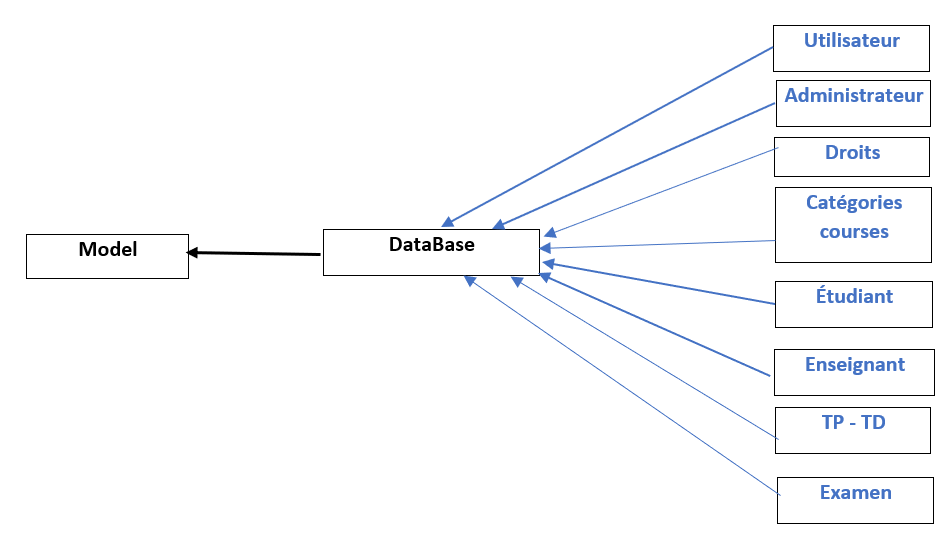
\includegraphics[width=13cm,height=6.80cm]{Larelation.jpg}
 	\caption{ La relation entre les différentes classes de l'application.}
 	\label{fig: La relation entre les différentes classes de l'application}
 \end{figure}
 \FloatBarrier
 \clearpage 
 La figure ci-dessous représente le diagramme de classes \cite{wiki:Diagramme_de_classes}:
 	
 
\begin{figure}[ht]
  \centering
  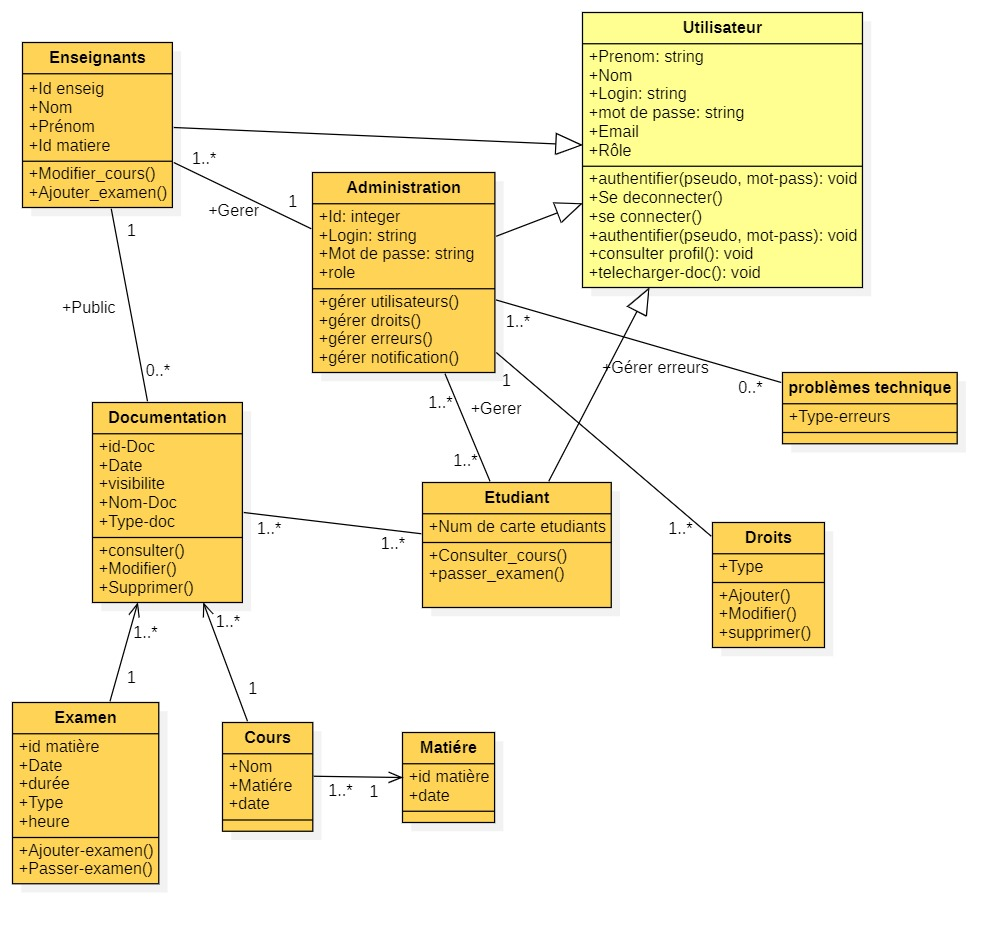
\includegraphics[width=18cm,height=16cm]{DiagrammedeclasseClassDiagram.jpg}
  \caption{Diagrammes de classes global.}
  \label{fig:UseCaseCatalogManager}
\end{figure}
\FloatBarrier
 \clearpage    

{\Large \color{cyan} Description des entités:}
 \smallskip
  \smallskip
   \smallskip
    \smallskip
     \smallskip
      \smallskip
       \smallskip
        \smallskip
         \smallskip
          \smallskip
           \smallskip
\begin{table}[h]
	\begin{itemize}
		
		\item \textit{\textbf{ Enseignants:}} L’utilisateur principal du module, il a accès à plusieurs fonctionnalités qui
		vont lui permettre de réussir le processus éducatif.
			\begin{itemize}	

			\item[$\star$] Faire un cours magistral :
			présentation, explication,
			argumentation et
			illustration d’un savoir
		


		\end{itemize}
	\end{itemize}
	\begin{center}
		\begin{tabular}{>{\begin{bf} } c <{\end{bf}}ccc}
			
			\rowcolor{-blue!20!red}Champs & \begin{bf}Types \end{bf} & \begin{bf}Contraintes\end{bf} & \\
			
			Id enseig & INT & PRIMARY KEY& \\
			
			Nom & VARCHAR(200)  & ---  &\\
			Prenom & VARCHAR(200)  & ---  &\\
			
			specialite  & VARCHAR & --- & \\
			specialite enseignement& INT& ---&\\

			email &VARCHAR(200)& UNIQUE&\\
telephone & VARCHAR(8) & ---& \\

			
		\end{tabular}
	\end{center}
	\caption{Tables  "Enseignants"}
	\label{Tables  "Enseignants"}
\end{table}
\smallskip
\smallskip
\smallskip
\begin{table}[h]
	
	\begin{itemize}
		
		\item \textit{\textbf{ Administration:}} On  le schéma de la base
		de données suivant :C'est la classe qui contient toutes les actions prises en charge
		par l'administrateur : 
	\end{itemize}
	\begin{center}
		\begin{tabular}{>{\begin{bf} } c <{\end{bf}}ccc}
			
			\rowcolor{-blue!20!red}Champs & \begin{bf}Types \end{bf} & \begin{bf}Contraintes\end{bf} & \\
			
			Id & INT & PRIMARY KEY& \\
			
			Nom &VARCHAR(200) & --- &\\
			prenom &VARCHAR(200) & --- &\\
			Mot de passe & VARCHAR(200)  & UNIQUE& \\
			
			role & VARCHAR(200) & UNIQUE  &\\
			email& VARCHAR(200)& UNIQUE &\\

		
			
		\end{tabular}
	\end{center}
	\caption{Tables  "Administration"}
	\label{mes belles tables}
\end{table}


\begin{table}[h]
	
	\begin{itemize}
		
		\item \textit{\textbf{ Etudiant:}} Le deuxième utilisateur du module avec des fonctionnalités facilitant la
		tâche de mémorisation.
	\end{itemize}
	\begin{center}
		\begin{tabular}{>{\begin{bf} } c <{\end{bf}}ccc}
			
			\rowcolor{-blue!20!red}Champs & \begin{bf}Types \end{bf} & \begin{bf}Contraintes\end{bf} & \\
			
			Num de carte etudiants & INT & PRIMARY KEY& \\
			nom & VARCHAR(200) & ---& \\
			prenom & VARCHAR(200) & ---& \\
			email &VARCHAR(200) &UNIQUE\\

			
			
			
			
		\end{tabular}
	\end{center}
	\caption{Tables  "Etudiant"}
	\label{mes belles table}
\end{table}

\begin{table}[h]
	
	\begin{itemize}
		
		\item \textit{\textbf{ TP/TD:}}C'est la classe qui contient toutes les TP et TD :
	\end{itemize}
	\begin{center}
		\begin{tabular}{>{\begin{bf} } c <{\end{bf}}ccc}
			
			\rowcolor{-blue!20!red}Champs & \begin{bf}Types \end{bf} & \begin{bf}Contraintes\end{bf} & \\
			
id &	INT(10)	&PRIMARY KEY& \\	
		\end{tabular}
	\end{center}
	\caption{Tables  "problèmes technique"}
	\label{Tables  "problèmes technique"s}
\end{table}














\begin{table}[h]
	
	\begin{itemize}
		
		\item \textit{\textbf{ Examen:}}  ça englobe toute les examens requis
	\end{itemize}
	\begin{center}
		\begin{tabular}{>{\begin{bf} } c <{\end{bf}}ccc}
			
			\rowcolor{-blue!20!red}Champs & \begin{bf}Types \end{bf} & \begin{bf}Contraintes\end{bf} & \\
			
			id &	INT(10)	&PRIMARY KEY& \\
			Date &VARCHAR(200) &---&\\
			durée & VARCHAR(200) &---&\\
			Type & VARCHAR(200) &---&\\
			heure & VARCHAR(200) &---&\\
			
		\end{tabular}
	\end{center}
	\caption{Tables  "Examen"}
	\label{Tables  "Examen"}
\end{table}










\begin{table}[h]
	
	\begin{itemize}
		
		\item \textit{\textbf{ Utilisateur:}}elle contient tous les utilisateurs du plateforme selon leur :
	\end{itemize}
	\begin{center}
		\begin{tabular}{>{\begin{bf} } c <{\end{bf}}ccc}
			
			\rowcolor{-blue!20!red}Champs & \begin{bf}Types \end{bf} & \begin{bf}Contraintes\end{bf} & \\
			id &INT &PRIMARY KEY&\\
pseudo& VARCHAR(200) &UNIQUE&\\
password& VARCHAR(200) &---&\\
privilege &VARCHAR(20) &---&\\


			
			
			
		\end{tabular}
	\end{center}
	\caption{Tables  "Utilisateur"}
	\label{Tables  "Utilisateur"}
\end{table}










\begin{table}[h]
	
	\begin{itemize}
		
		\item \textit{\textbf{ Cours:}}
		ca englobe toute les cours nécessaires au processus d'enseignement à distance
	\end{itemize}
	\begin{center}
		\begin{tabular}{>{\begin{bf} } c <{\end{bf}}ccc}
			
			\rowcolor{-blue!20!red}Champs & \begin{bf}Types \end{bf} & \begin{bf}Contraintes\end{bf} & \\

		id &	INT(10)	&PRIMARY KEY& \\
		
		user id&	INT(11)&---& \\
		
		category id&	INT(11)&---& \\
		
		title	&varchar(255)&---& \\	
		
		sub title&	varchar(255)&---& \\		
		
		description	&longtext	&---& \\
		
		about instructor&	longtext&---& \\	
		
		playlist url&	varchar(255)&---& \\	
		
		photo&	varchar(255)&---& \\	
		
		promo video url&	varchar(255)&---& \\	
		
		tags&	varchar(255)&---& \\	
		
		creator status&	INT(11)	&---& \\		
		
		admin status&	INT(11)	&---& \\	
		
		what will student learn&	longtext	&---& \\
		
		target student&	longtext&---& \\		
		
		requirements&	longtext&---& \\	
		
		discount price&	double(10,2)&---& \\		
		
		actual price&	double(10,2)	&---& \\	
		
		view count&	INT(11)	&---& \\		
		
		subscriber count&	int(11)	&---& \\
			
			
		\end{tabular}
	\end{center}
	\caption{Tables  "Cours"}
	\label{Tables  "Cours"}
\end{table}

\begin{table}[h]
    \begin{itemize}
      \item \textit{\textbf{ Catégorie Matiére:}}ca englobe toute les Matiéres
	\end{itemize}
	\begin{center}
		\begin{tabular}{>{\begin{bf} } c <{\end{bf}}ccc}
			
			\rowcolor{-blue!20!red}Champs & \begin{bf}Types \end{bf} & \begin{bf}Contraintes\end{bf} & \\
  

id 	&INT(10)	&PRIMARY KEY& \\	

name&	varchar(255)&---& \\	

description	&longtext&---	& \\

categories photos&	longtext&---& \\	

view count	&INT(11)&---	& \\		


			
			
		\end{tabular}
	\end{center}
	\caption{Tables  "Catégorie Matiére"}
	\label{Catégorie Matiére}
\end{table}
\clearpage 
\begin{table}[h]
	
	\begin{itemize}
		
		\item \textit{\textbf{ Droits:}}c'est la classe qui contient les droits attribués aux plateforme par
		l’administrateur ainsi la suppression ou l’ajout de certains privilèges.
	\end{itemize}
	\begin{center}
		\begin{tabular}{>{\begin{bf} } c <{\end{bf}}ccc}
			
			\rowcolor{-blue!20!red}Champs & \begin{bf}Types \end{bf} & \begin{bf}Contraintes\end{bf} & \\
			
			id & INT & PRIMARY KEY& \\
			titre & VARCHAR(200) & UNIQUE& \\
		\end{tabular}
	\end{center}
	\caption{Tables  "Droits"}
	\label{mTables  "Droits"}
\end{table}


\FloatBarrier

\section{Conclusion}
Le but de ce chapitre était de définir et d’analyser l’ensemble des besoins fonctionnels  de notre solution. Cette étape est primordiale dans le développement d’un projet informatique puisque elle nous permet de définir le périmètre fonctionnel du projet, et de garantir la couverture de l’ensemble des fonctionnalités recensées.
